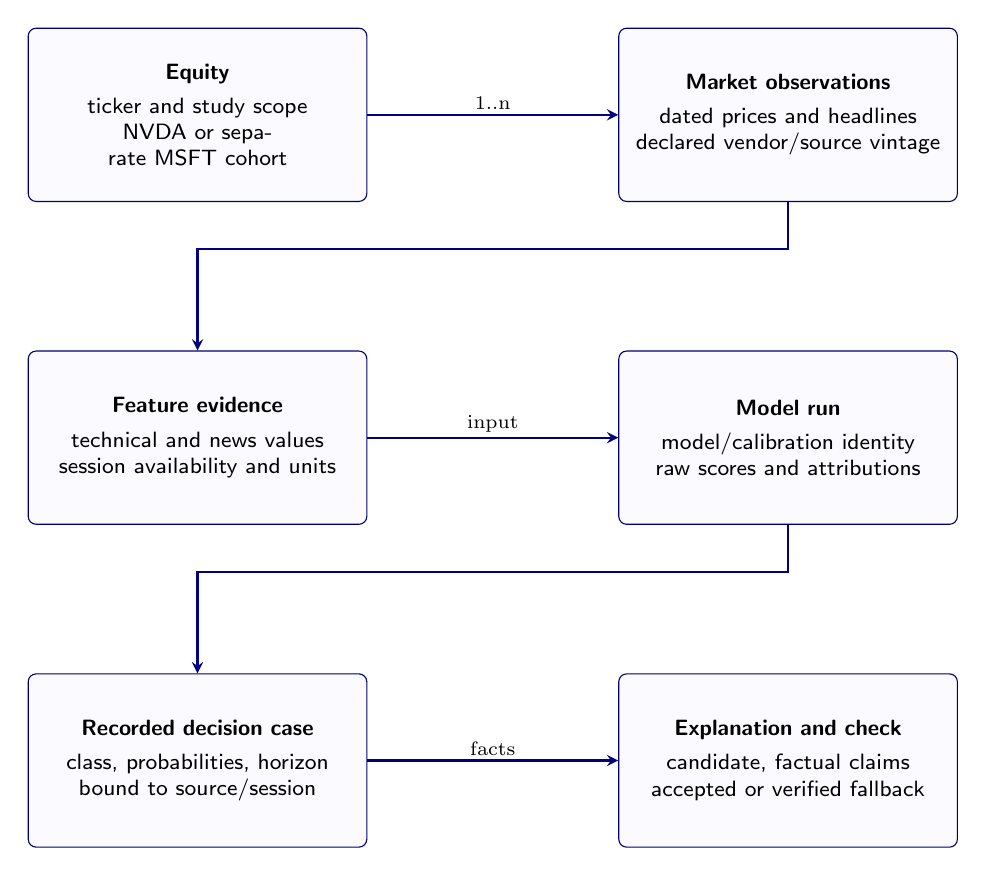
\begin{tikzpicture}[x=1mm,y=1mm,box/.style={draw=blue!45!black,fill=blue!2,rounded corners=1mm,align=center,text width=39mm,minimum height=22mm,inner sep=2mm,font=\sffamily\footnotesize},link/.style={->,>=stealth,draw=blue!50!black,thick}]
\node[box] (equity) at (30,115) {\textbf{Equity}\\[1mm]ticker and study scope\\NVDA or separate MSFT cohort};
\node[box] (observations) at (105,115) {\textbf{Market observations}\\[1mm]dated prices and headlines\\declared vendor/source vintage};
\node[box] (features) at (30,74) {\textbf{Feature evidence}\\[1mm]technical and news values\\session availability and units};
\node[box] (model) at (105,74) {\textbf{Model run}\\[1mm]model/calibration identity\\raw scores and attributions};
\node[box] (decision) at (30,33) {\textbf{Recorded decision case}\\[1mm]class, probabilities, horizon\\bound to source/session};
\node[box] (explanation) at (105,33) {\textbf{Explanation and check}\\[1mm]candidate, factual claims\\accepted or verified fallback};
\draw[link] (equity.east) -- (observations.west) node[pos=.5,above,fill=white,inner sep=.5mm,font=\scriptsize]{1..n};
\draw[link] (observations.south) -- ++(0,-6) -| (features.north);
\draw[link] (features.east) -- (model.west) node[pos=.5,above,fill=white,inner sep=.5mm,font=\scriptsize]{input};
\draw[link] (model.south) -- ++(0,-6) -| (decision.north);
\draw[link] (decision.east) -- (explanation.west) node[pos=.5,above,fill=white,inner sep=.5mm,font=\scriptsize]{facts};
\end{tikzpicture}
